% Copyright Ben Paul Wise. All Rights Reserved.
% The full-page locator map before each section of figures: the standard sheet with the area of the section's
% figures boxed in black.  Shared by circling_dragons_map_and_rules_V3.tex and maneuver_studies_75km.tex; needs
% graphicx and tikz.  The boxes are generated by map_graphics/xml/tools/cd/illustrate.py (locator-boxes.tex).
% The map is set once in a box, so the PDF carries one copy of the image however many locators there are.
% Copyright Ben Paul Wise. All Rights Reserved.
% Generated by map_graphics/xml/tools/cd/illustrate.py; do not edit.  The area each section's figures show
% on the standard sheet, as a TikZ rectangle in fractions of the sheet (x from the left, y from the bottom).
\def\cdboxIchigo{(0.1568,0.0943) rectangle (0.5986,0.6013)}   % 1-ichigo-setup
\def\cdboxReflux{(0.1568,0.0943) rectangle (0.5986,0.6013)}   % 2-reflux-setup
\def\cdboxAugust{(0.3402,0.5942) rectangle (0.9654,0.9891)}   % 3-august-setup
\def\cdboxRace{(0.2587,0.4484) rectangle (0.8432,0.9241)}   % 4-race-setup
\def\cdboxChangsha{(0.3198,0.2297) rectangle (0.4968,0.3746)}   % a1-changsha-position
\def\cdboxHengyang{(0.2995,0.1568) rectangle (0.4764,0.3225)}   % b1-hengyang-position
% Copyright Ben Paul Wise. All Rights Reserved.

\newsavebox{\cdmapbox}
\AtBeginDocument{\sbox{\cdmapbox}{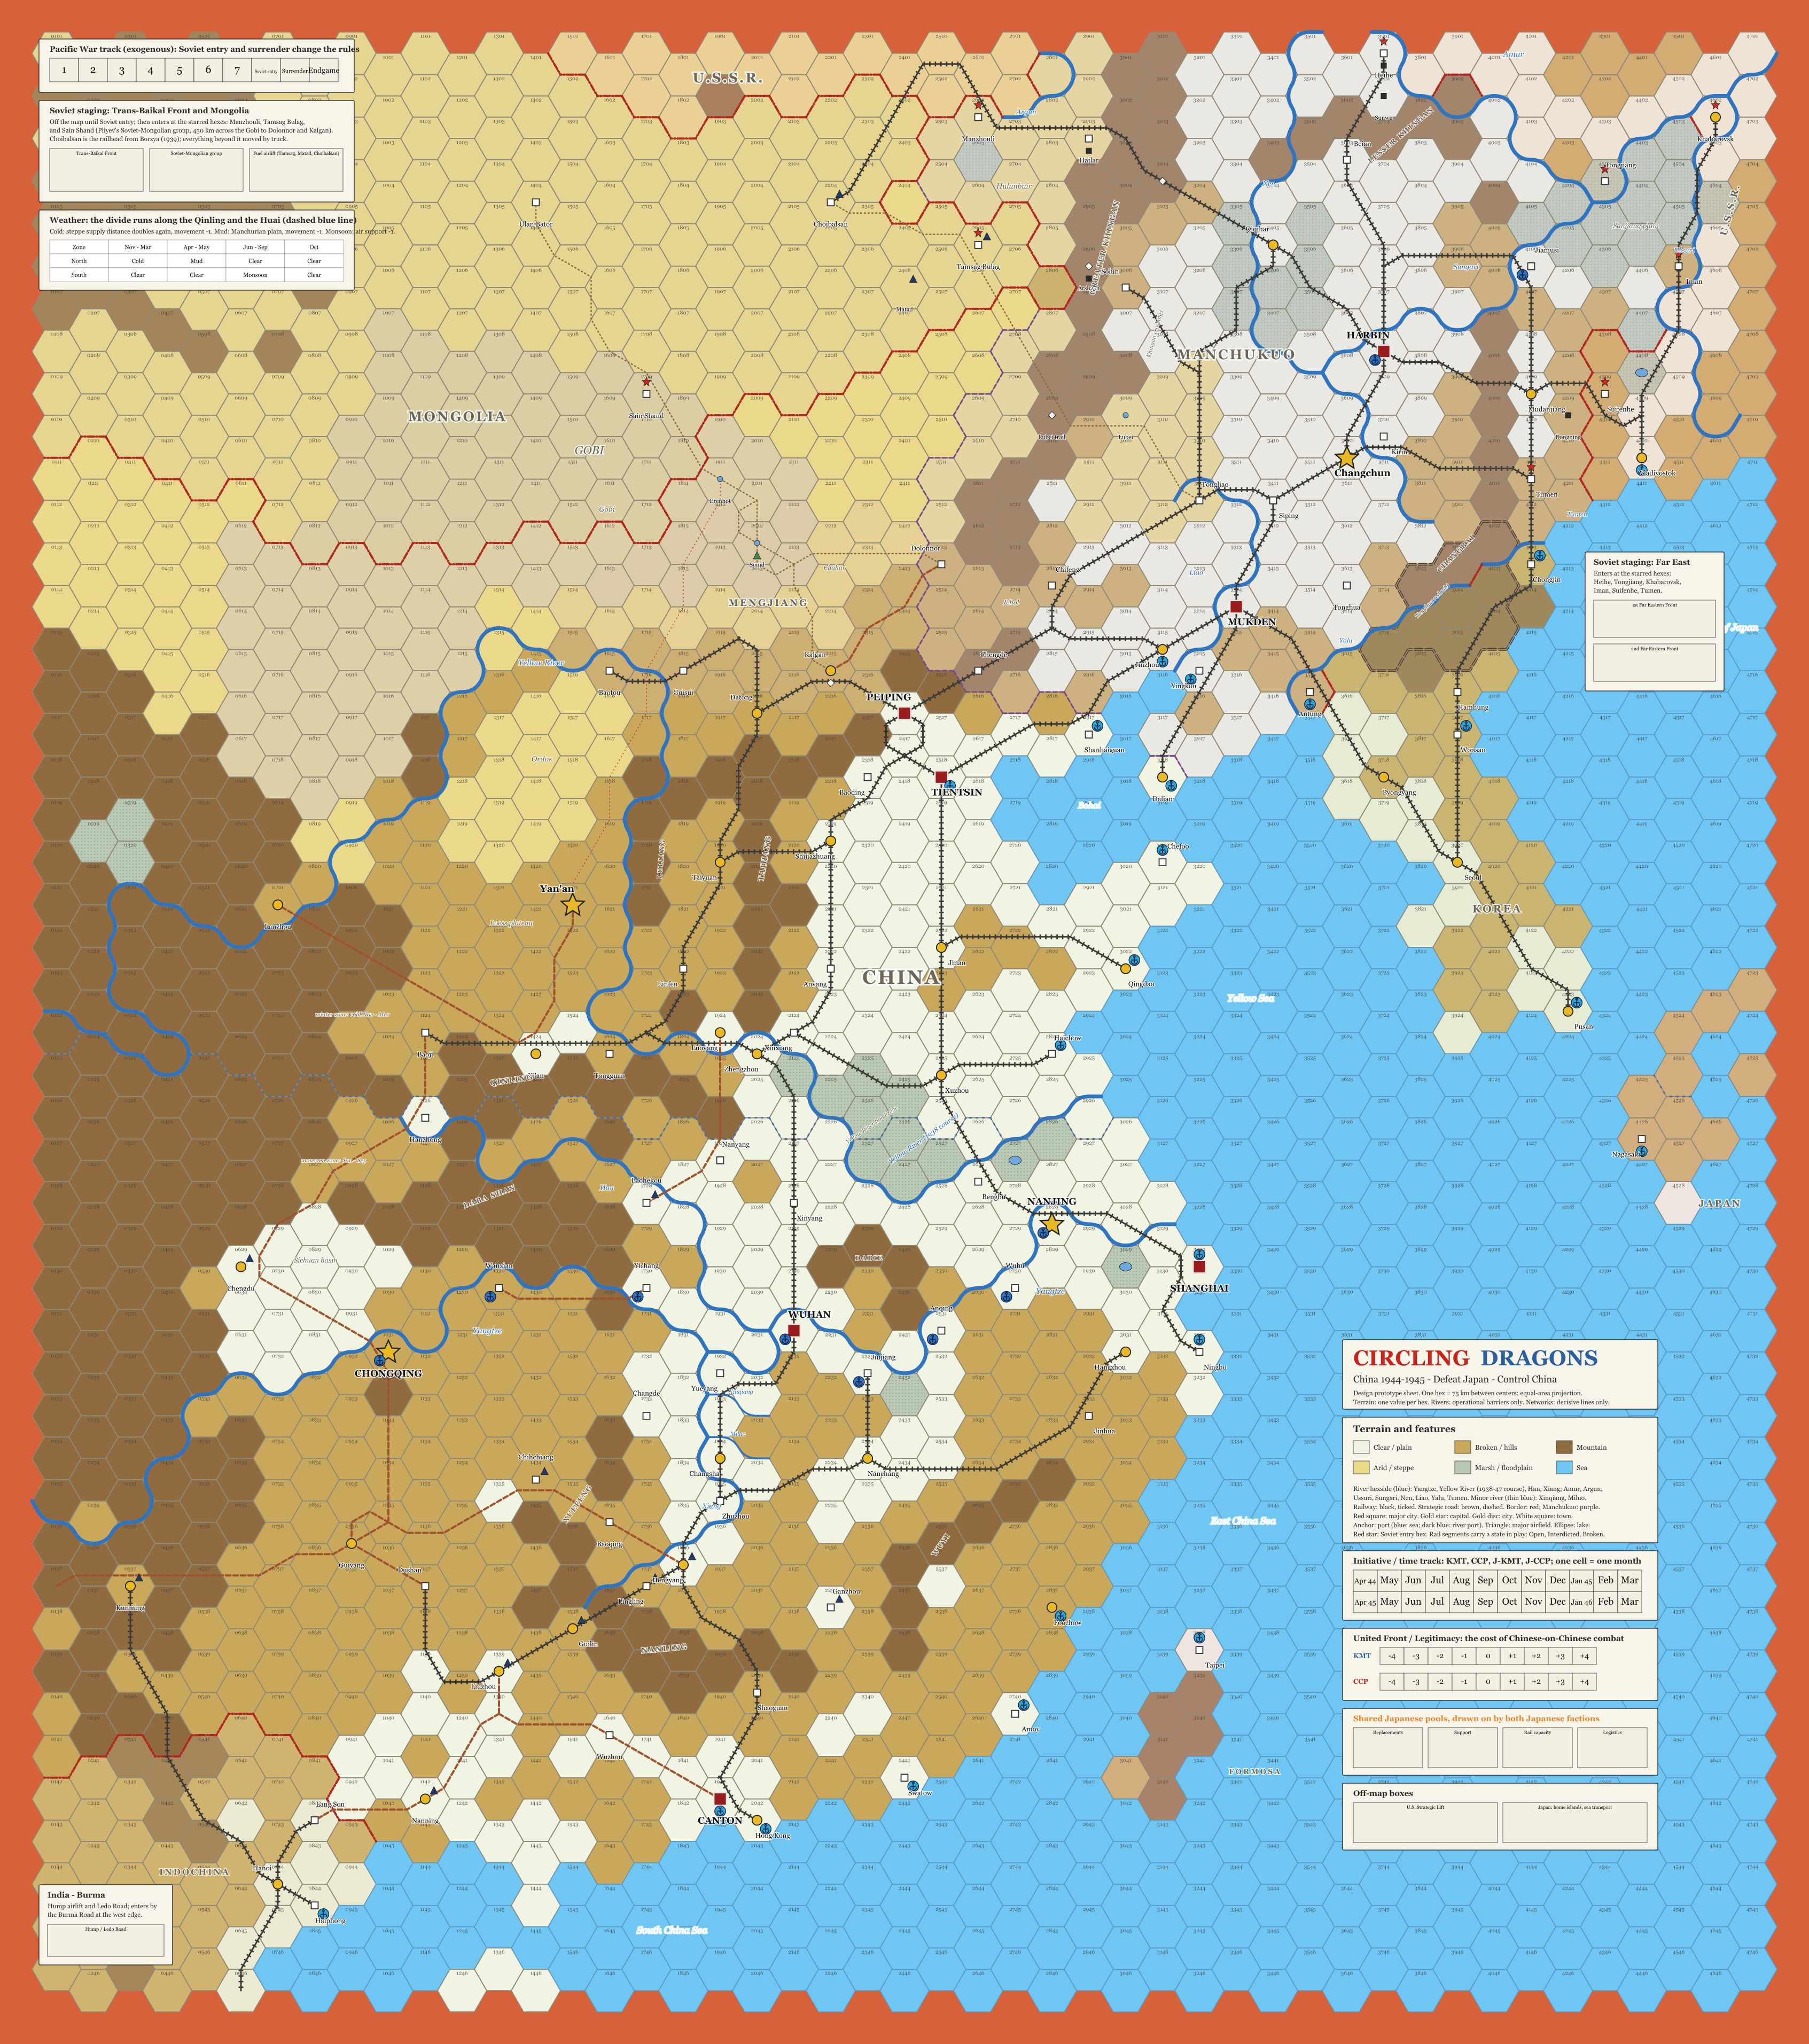
\includegraphics[width=\textwidth,height=.84\textheight,keepaspectratio]{../map_graphics/xml/circling-dragons.png}}}
\newcommand{\locator}[2]{%
  \clearpage
  \begin{figure}[p]\centering
  \begin{tikzpicture}
    \node[anchor=south west,inner sep=0] (map) at (0,0) {\usebox{\cdmapbox}};
    \begin{scope}[x={(map.south east)},y={(map.north west)}]
      \draw[white,line width=5pt] #1;
      \draw[black,line width=2.6pt] #1;
    \end{scope}
  \end{tikzpicture}
  \caption{#2}
  \end{figure}
  \clearpage}
% Copyright Ben Paul Wise. All Rights Reserved.
